% ======================================================================
% TC-ViTok --- ICONIP 2026 submission
% Springer LLNCS class (Lecture Notes in Computer Science)
% ======================================================================
\documentclass[runningheads]{llncs}

\usepackage[T1]{fontenc}
\usepackage[utf8]{inputenc}
\usepackage{lmodern}
\usepackage[activate={true,nocompatibility},final,expansion=false]{microtype}
\usepackage{graphicx}
\usepackage{amsmath}
\usepackage{amssymb}
\usepackage{booktabs}
\usepackage{xcolor}
\usepackage{pifont}
\usepackage{caption}
\usepackage{subcaption}
\usepackage{tikz}
\usetikzlibrary{arrows.meta}
\usepackage{hyperref}
\renewcommand\UrlFont{\color{blue}\rmfamily}
\urlstyle{rm}
\captionsetup{font=small,skip=2pt}
\setlength{\textfloatsep}{8pt plus 1pt minus 2pt}
\setlength{\floatsep}{6pt plus 1pt minus 2pt}
\setlength{\intextsep}{6pt plus 1pt minus 2pt}

\newcommand{\vcoarse}{\mathbf{v}_{c}}
\newcommand{\vfine}{\mathbf{v}_{f}}
\newcommand{\qemb}{\mathbf{q}}
\newcommand{\sN}{\mathbf{s}_N}
\newcommand{\vsel}{\mathbf{v}_{\mathrm{sel}}}
\newcommand{\vunsel}{\mathbf{v}_{\mathrm{unsel}}}
\newcommand{\vmerged}{\mathbf{v}_{\mathrm{merged}}}
\newcommand{\keff}{k_{\mathrm{eff}}}
\newcommand{\kmax}{k_{\max}}
\newcommand{\Tosc}{T_{\mathrm{osc}}}
\newcommand{\etasel}{\eta_{\mathrm{sel}}}
\newcommand{\etalora}{\eta_{\mathrm{LoRA}}}
\newcommand{\lbb}{\lambda_b}
\newcommand{\Lvqa}{\mathcal{L}_{\mathrm{VQA}}}

\begin{document}
\setlength{\abovedisplayskip}{5pt}
\setlength{\belowdisplayskip}{5pt}
\setlength{\abovedisplayshortskip}{3pt}
\setlength{\belowdisplayshortskip}{3pt}

% ----------------------------------------------------------------------
\title{Why Jointly Learned Pre-LLM\\
       Visual Token Selectors Can Fail:\\
       A Diagnostic Case Study}
\titlerunning{Why Pre-LLM Visual Token Selectors Can Fail}

\author{Muhammad Ali Shah\inst{1} \and Talha Hassan Ul Haq\inst{1}}
\authorrunning{M.\,A.\,Shah and T.\,H.\,Ul\,Haq}
\institute{Lahore University of Management Sciences (LUMS),
           Lahore, Pakistan\\
           \email{\{27100172, 27100306\}@lums.edu.pk}}

\maketitle
% ----------------------------------------------------------------------

\begin{abstract}
Pre-LLM visual-token compression can save the full visual prefill cost
of a vision-language model if a small selector can learn which image
tokens the LLM needs for the current question. We test this idea with
\textsc{TC-ViTok}, a query-conditioned selector that compresses
$576$ CLIP patches to $k{=}144$ before LLaVA-1.5-7B LoRA training.
The result is negative but controlled: the learned selector loses by
$4.1/3.4/7.4$ points on VQAv2/GQA/POPE to a compute-matched
no-compression LoRA-576 reference, and it fails to surpass the strongest
question-blind trivial baseline on any of the five evaluated
benchmarks. We use this
failure as a diagnostic case study rather than proposing
\textsc{TC-ViTok} as a compression method. In this stack we identify
three failure-mode (FM) hypotheses: coupled selector--adapter oscillation,
adaptive-budget collapse, and warm-start dependence. We describe
engineering interventions that stabilise training sufficiently for diagnosis: a
$\tau$-independent straight-through gradient route, a parameter-free
informative token merge that removes a trainable bridge, and a
three-stage warm-start curriculum. Seed-42 adaptive-budget
continuations identify a non-collapsed region at least through
$\lbb{=}0.15$, with independent seed-7 replications confirming collapse
at $\lbb{=}0.03$ and stability at $\lbb{=}0.08$, $0.10$, and $0.15$;
$\lbb{=}0.20$ shows stronger budget pressure in a single seed.
Supporting probes do not recover single-token ablation
importance from CLIP/DINOv2 features under the tested linear/MLP
probes and sample sizes, while coordinate controls are positive.
Evidence is primarily from one LLaVA-1.5-7B stack; a Qwen2-VL-7B
portability attempt failed to reach non-trivial task accuracy and is
not used as validation.

\keywords{Vision-Language Models \and Visual Token Compression
\and Training Dynamics \and Co-Adaptation \and Straight-Through Estimator
\and Query-Conditioned Selection.}
\end{abstract}

% ======================================================================
\section{Introduction}
\label{sec:intro}

Modern vision-language models (VLMs) such as
LLaVA-1.5~\cite{liu2024llava} attach a large language model (LLM) to a
frozen CLIP~\cite{radford2021clip} vision encoder. The encoder maps a
$336{\times}336$ image to $N{=}576$ patch tokens which are prepended to
the tokenised question and fed into the LLM. Because LLM attention cost
scales quadratically with sequence length, these visual tokens dominate
prefill FLOPs, and the budget is set by image resolution rather than by
what the question requires.

A natural design point is a \emph{trainable, query-conditioned pre-LLM}
compression module that selects $k\!\ll\!N$ tokens before the LLM runs.
Pre-LLM placement saves the full prefill cost (unlike mid-LLM
pruning~\cite{chen2024fastv,zhang2025sparsevlm}), and query conditioning
lets the budget concentrate on the patches relevant to the current
question (unlike query-agnostic approaches~\cite{bolya2022token,liang2022evit,shang2024llava}).
The intuitive hope is simple: the selector should learn to keep the
image patches the LLM needs for the current question. The supervision
is, however, highly indirect. The selector receives no token-level
labels; gradient arrives only after its selected tokens pass through a
frozen projector and a 32-layer LLM whose LoRA~\cite{hu2022lora} adapters are
simultaneously changing. The selector therefore trains against a
moving downstream model rather than a fixed target, and the LLM
adapters in turn train against a moving selector. This is a coupled
two-timescale optimisation problem: both parameter groups minimise the
same VQA loss, but each changes the gradient field seen by the other.

We built \textsc{TC-ViTok} to test the natural idea above, and found
it fails in a strong and informative way. The learned selector loses
by $4.1/3.4/7.4$ points on VQAv2/GQA/POPE to a matched no-compression
LoRA-576 reference, \emph{and} fails to surpass the strongest of three
trivial token-selection controls: uniform random drop, uniform grid
every $4$th patch, and CLS-attention top-$k$ on CLIP's last layer,
on every benchmark we measure. The gap to trivial selectors is the
phenomenon this paper explains, not a peripheral limitation: if a
jointly trained query-conditioned selector cannot beat selectors that
do not see the question at all, end-task supervision alone is not
reliably discovering token importance in this stack. We therefore use
TC-ViTok as a controlled diagnostic substrate rather than as a
proposed compression method, and the paper's contribution is the
structured account of \emph{why} the gap appears.
The negative outcome is not a foregone conclusion: query-conditioned
compression modules can succeed when trained with stronger priors or
supervision~\cite{li2023blip2,zhang2025sparsevlm,li2025qgvtc}, and
one would expect a query-conditioned selector to beat query-blind
baselines at the same budget. Our result isolates where that
conjecture fails under matched LoRA training and end-task supervision
alone.

\paragraph{Contributions.}
\begin{itemize}
\setlength{\itemsep}{0pt}
\setlength{\parsep}{0pt}
\setlength{\topsep}{2pt}
\item \textbf{Controlled negative result.} Against the compute-matched
\textsc{LoRA-576} reference and three trivial selectors, the
learned query-conditioned selector fails to surpass the strongest
question-blind trivial selector on any evaluated benchmark.
\item \textbf{Single-stack diagnostic case study.} We characterise
three failure modes (FM): coupled selector--adapter oscillation,
adaptive BudgetPredictor collapse, and warm-start dependence. Each has a
mechanism, signature, and reproduction protocol; we do not claim
architectural universality.
\item \textbf{Engineering interventions and diagnostics.} We use a
$\tau$-independent straight-through gradient route (Eq.~\ref{eq:taufix}),
a parameter-free informative token merge, and a three-stage warm-start
curriculum. We also report query-agnostic convergence as
trajectory-level evidence.
\item \textbf{Falsifiable reproduction protocols.} We give concrete
FM1--FM3 tests for independent stacks, including a distillation-based
falsification criterion for FM3.
\end{itemize}

% ======================================================================
\section{Related Work}
\label{sec:related}

\paragraph{Query-agnostic visual token compression.}
ToMe~\cite{bolya2022token} merges similar tokens via bipartite
matching. DynamicViT~\cite{rao2021dynamicvit} learns Gumbel-Softmax
drop masks distilled from a teacher. EViT~\cite{liang2022evit} ranks
tokens by CLS-attention and fuses low-importance ones.
PruMerge~\cite{shang2024llava} prunes by CLS rank and merges pruned
tokens into nearest neighbours. FastV~\cite{chen2024fastv} prunes
inside the LLM at layer 2, after visual information has mixed into
the text stream. These methods avoid training or rely on strong
priors (CLS, layer-2 attention) rather than learn query-aware
routing.

\paragraph{Query-aware compression.}
BLIP-2~\cite{li2023blip2} uses cross-attention between a fixed bank of
learned queries and visual tokens. SparseVLM~\cite{zhang2025sparsevlm}
sparsifies inside the LLM using text-to-visual attention with per-layer
recycling. QG-VTC~\cite{li2025qgvtc} injects the question into the
encoder and compresses progressively within it.
FocusLLaVA~\cite{zhu2024focusllava} performs coarse-to-fine
instruction-guided selection inside the LLM. No prior work we are aware
of combines (a) explicit per-question conditioning, (b) pre-LLM
placement on frozen features, and (c) per-sample adaptive budget in the
setting studied here; we position \textsc{TC-ViTok} as that combination,
primarily so we can study its training dynamics.

\paragraph{Differentiable discrete selection.}
Gumbel-Softmax~\cite{jang2017categorical,maddison2017concrete} and
straight-through estimators~\cite{bengio2013estimating} are standard
tools for learning subset selectors;
AdaViT~\cite{meng2022adavit} extends these to per-sample budgets. We
adopt Gumbel-Sigmoid for independent binary decisions and use a
$\tau$-independent additive gradient route (Section~\ref{sec:ste}) to
avoid low-temperature gradient starvation in our setting.

\paragraph{Training-dynamics perspective.}
Unlike inference-only compression, our setting jointly trains a pre-LLM
selector with LoRA adapters. This motivates the two-timescale
optimisation~\cite{borkar1997stochastic,konda2004convergence} and
curriculum-learning~\cite{bengio2009curriculum} lens used later; the
compute-matched \textsc{LoRA-576} control isolates compression from
fine-tuning effects.

% ======================================================================
\section{Method}
\label{sec:method}

\subsection{Problem Setup and the Co-Adaptation Loop}
\label{sec:co-adaptation}

Given image $\mathbf{I}$ and question $\mathbf{Q}$, we learn a policy
$\pi_\phi(\mathbf{I},\mathbf{Q})\!\to\!\mathcal{S}\!\subseteq\!\{1,\ldots,N\}$
with $|\mathcal{S}|{=}k$; the LLM receives only the $k$ selected
tokens. Selector parameters $\phi$ and LLM-adapter parameters
$\theta_\text{LoRA}$ are jointly trained against the VQA loss:
\begin{equation}
\Lvqa(\phi,\theta_\text{LoRA})
= \mathbb{E}_{(I,Q,y)}
\left[-\log p_\theta\!\left(y\,\middle|\,\pi_\phi(I,Q)\right)\right].
\label{eq:vqa-loss}
\end{equation}
This induces a coupled gradient circuit: selector updates shift the
LLM input distribution, LoRA updates shift the gradient field the
selector sees, and both groups respond to a moving target. The setting
is cooperative rather than adversarial: both groups minimise the
same VQA loss. We use GAN limit cycles only as an analogy for
moving-target optimisation, not as a formal reduction. A closer lens is
two-timescale stochastic approximation and bilevel instability
\cite{borkar1997stochastic,konda2004convergence}; we cite these as the
appropriate formal lens, not as a convergence guarantee for our
nonconvex VLM setting. We observe limit-cycle-like trajectories
empirically (Section~\ref{sec:fm1}), motivating three design choices:
parameter-free recovery (no learnable bridge, Section~\ref{sec:merge}),
warm-freezing LoRA (break the loop in time,
Section~\ref{sec:training}), and adaptive-budget training only on a
converged base (Section~\ref{sec:warmstart}).

\subsection{Architecture}
\label{sec:tpn}

We use three frozen pretrained encoders: DINOv2-S~\cite{oquab2023dinov2}
on a $98{\times}98$ crop produces $\vcoarse\!\in\!\mathbb{R}^{49\times 384}$
that the selector cross-attends; CLIP ViT-B/32~\cite{radford2021clip}
encodes the question into $\qemb\!\in\!\mathbb{R}^{512}$; and CLIP
ViT-L/14~\cite{radford2021clip} produces the LLM input
$\vfine\!\in\!\mathbb{R}^{576\times 1024}$ (aligned to LLaVA-1.5's
projector). No gradient flows into any encoder. Thus the TPN consumes
$(\qemb,\vcoarse)$ and scores the 576 CLIP-L tokens $\vfine$ before
selection, merge, and the LLaVA projector.

\begin{figure}[t]
\centering
\resizebox{0.96\textwidth}{!}{%
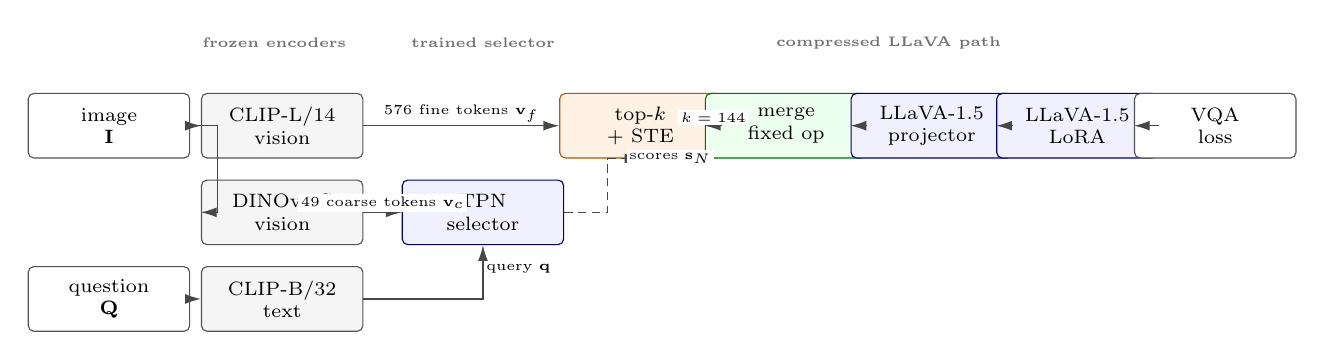
\begin{tikzpicture}[
font=\scriptsize,
module/.style={
    draw=black!68,
    rounded corners=2pt,
    align=center,
    minimum height=8.2mm,
    minimum width=20.5mm,
    inner sep=2.4pt
},
input/.style={module, fill=white},
frozen/.style={module, fill=black!4},
train/.style={module, fill=blue!6, draw=blue!48!black},
op/.style={module, fill=orange!10, draw=orange!70!black},
fixed/.style={module, fill=green!7, draw=green!45!black},
tag/.style={font=\tiny\bfseries, text=black!55},
arr/.style={-{Latex[length=2.0mm,width=1.25mm]}, line width=.45pt, draw=black!72},
darr/.style={arr, densely dashed}
]

\node[tag] at (2.10, 2.15)  {frozen encoders};
\node[tag] at (4.75, 2.15)  {trained selector};
\node[tag] at (9.90, 2.15)  {compressed LLaVA path};

\node[input]  (img)   at (0.00,  1.10) {image\\$\mathbf{I}$};
\node[input]  (ques)  at (0.00, -1.10) {question\\$\mathbf{Q}$};

\node[frozen] (clipv) at (2.20,  1.10) {CLIP-L/14\\vision};
\node[frozen] (dino)  at (2.20,  0.00) {DINOv2-S\\vision};
\node[frozen] (clipt) at (2.20, -1.10) {CLIP-B/32\\text};

\node[train]  (tpn)   at (4.75,  0.00) {TPN\\selector};
\node[op]     (topk)  at (6.75,  1.10) {top-$k$\\+ STE};
\node[fixed]  (merge) at (8.60,  1.10) {merge\\fixed op};
\node[train]  (proj)  at (10.45, 1.10) {LLaVA-1.5\\projector};
\node[train]  (llm)   at (12.30, 1.10) {LLaVA-1.5\\LoRA};
\node[input]  (loss)  at (14.05, 1.10) {VQA\\loss};

\draw[arr] (img.east)  -- (clipv.west);
\draw[arr] (img.east) -- ++(0.35,0) |- (dino.west);
\draw[arr] (ques.east) -- (clipt.west);

\draw[arr]
(clipv.east) -- (topk.west)
node[
    above,
    midway,
    font=\tiny,
    fill=white,
    inner sep=1pt
]
{$576$ fine tokens $\vfine$};

\draw[arr]
(dino.east) -- (tpn.west)
node[
    above,
    midway,
    font=\tiny,
    fill=white,
    inner sep=1pt
]
{$49$ coarse tokens $\vcoarse$};

\draw[arr]
(clipt.east) -| (tpn.south)
node[
    pos=0.78,
    right,
    font=\tiny,
    fill=white,
    inner sep=1pt
]
{query $\qemb$};

\draw[darr]
(tpn.east) -- ++(0.55,0) |- (topk.south)
node[
    pos=0.78,
    right,
    font=\tiny,
    fill=white,
    inner sep=1pt
]
{scores $\sN$};

\draw[arr]
(topk.east) -- (merge.west)
node[
    above,
    midway,
    font=\tiny,
    fill=white,
    inner sep=1pt
]
{$k=144$};

\draw[arr] (merge.east) -- (proj.west);
\draw[arr] (proj.east)  -- (llm.west);
\draw[arr] (llm.east)   -- (loss.west);
\end{tikzpicture}%
}
\caption{\textsc{TC-ViTok} dataflow. Frozen encoders provide fine
CLIP tokens, coarse DINOv2 features, and the text query. The TPN
consumes only $(\qemb,\vcoarse)$, scores the 576-token CLIP grid, and
the selected tokens pass through fixed merge, the LLaVA-1.5 projector,
and LoRA-adapted decoding. Gray nodes are frozen, blue nodes are
trained, green is parameter-free, orange is discrete selection, and
dashed arrows carry selector scores.}
\label{fig:architecture}
\end{figure}

The \emph{Tokenisation Policy Network} (TPN, ${\approx}887$K parameters)
cross-attends $\qemb$ over $\vcoarse$ with four heads to produce a context vector $\mathrm{ctx}\!\in\!\mathbb{R}^{384}$
and head-averaged spatial weights
$\boldsymbol{\alpha}\!\in\!\mathbb{R}^{49}$. A small score MLP on
$[\mathrm{ctx};\boldsymbol{\alpha}]$ emits 49 coarse scores, bilinearly
upsampled to a $24{\times}24$ grid and \emph{instance-normalised} to
$\mu{=}0,\sigma{=}1$ per sample. Instance normalisation is necessary:
without it Adam pushes scores to ${\pm}100$ within $\sim$1K steps and
Gumbel noise becomes negligible; \texttt{tanh} (saturation) and batch
norm (single-sample inference) failed analogously.

\subsection{Gumbel-Sigmoid STE with \texorpdfstring{$\tau$}{tau}-Independent Correction}
\label{sec:ste}

Token selection is a discrete top-$k$ operation. We use Gumbel-Sigmoid
STE for independent binary subset selection over 576 positions. With
$\mathbf{g}\!\sim\!\mathrm{Gumbel}(0,1)$ and $\tau$ annealed linearly
$1.0\!\to\!0.3$, selection is
\begin{equation}
\begin{aligned}
\mathbf{n} &= \sN + \mathbf{g}, &
\mathbf{m}_{\mathrm{soft}} &= \sigma(\mathbf{n}/\tau),\\
\mathrm{idx} &= \mathrm{topk}(\mathbf{n}, k), &
\mathbf{m}_{\mathrm{STE}} &=
\mathbf{m}_{\mathrm{hard}}
- \mathbf{m}_{\mathrm{soft}}.\mathrm{detach}()
+ \mathbf{m}_{\mathrm{soft}} .
\end{aligned}
\label{eq:gumbel-ste}
\end{equation}
The gradient flows through $\mathbf{m}_{\mathrm{soft}}$.

At low $\tau$, $\mathbf{m}_{\mathrm{soft}}$ saturates and
$\partial \mathbf{m}_{\mathrm{soft}}/\partial \sN\!\approx\!0$ for
$|\sN[i]|\!>\!1$, killing the gradient to the selector. Letting
$\mathbf{c}{=}\mathrm{gather}(\sN,\text{idx})$, we apply
\begin{equation}
\vsel \leftarrow \vsel \odot \bigl(1 + \mathbf{c} - \mathbf{c}.\mathrm{detach}()\bigr).
\label{eq:taufix}
\end{equation}
Forward: $\mathbf{c}{-}\mathbf{c}.\mathrm{detach}(){=}\mathbf{0}$, so
$\vsel$ is unchanged. Backward: for selected position $j$,
$\partial \Lvqa/\partial \sN[j]{=}\sum_d (\partial \Lvqa/\partial \vsel[j,d])\,\vsel[j,d]$,
a dot product between the VQA gradient and the visual features at $j$
that can remain non-zero even when the sigmoid surrogate saturates. In
policy-gradient terms, this is a biased straight-through gradient route
rather than an unbiased estimator of the discrete subset objective; we
use it as an engineering device to keep selected-token task gradients
connected to selector scores. In a matched 50K-step Phase-1 ablation
using the same joint-training setup, disabling Eq.~\ref{eq:taufix}
worsens final validation next-token-prediction (NTP) loss from
$0.3511$ to $0.3846$ (lower is better), directly validating the
correction at the task-loss level. A matched 12K-step Phase-1
joint-training diagnostic run also shows the intended gradient effect:
at $\tau{\approx}0.10$, the final TPN gradient norm is $0.0324$ with
Eq.~\ref{eq:taufix} versus $0.0030$ without it, while LoRA gradient norms remain comparable
($0.4091$ vs.\ $0.4277$). A matched no-correction diagnostic with a
higher temperature floor ($\tau_\mathrm{min}{=}0.5$) gives a final TPN
gradient norm of only $0.0029$ and validation NTP loss $0.4069$ at 12K
steps, indicating that the additive route provides gradient connectivity
not recovered by this simple temperature-floor adjustment. The
$0.4069$ loss is a 12K diagnostic value and is not directly comparable
to the 50K no-correction loss; the matched evidence here is the TPN
gradient norm.

\subsection{Informative Token Merge (Parameter-Free)}
\label{sec:merge}

Hard dropping of the $N{-}k{=}432$ unselected tokens discards their
context. We route them into selected tokens via cosine similarity
weighted by TPN scores, with normalisation
$\tilde{A}_{ij}{=}w_i A_{ij}/\sum_{i'} w_{i'} A_{i'j}$ where
$A_{ij}$ is a row-softmax over cosine similarity at temperature
$\tau_m$ and $w_i$ is a column-softmax over unselected-token scores:
\begin{equation}
\vmerged = \vsel + \beta\,\tilde{A}^\top \vunsel, \qquad \beta{=}0.3,\; \tau_m{=}0.1.
\end{equation}
The merge has \emph{zero new parameters}, eliminates co-adaptation
risk with LoRA by construction, and preserves the token count $k$
between training and evaluation. A previous family of eight
\emph{trainable} pooler configurations displayed the closed-loop
oscillation diagnosed in Section~\ref{sec:fm1}; the parameter-free
merge structurally severs one edge of the gradient circuit and
eliminates those failures.

\subsection{Adaptive Budget and Training Curriculum}
\label{sec:training}

A small ${\approx}25$K-parameter \emph{BudgetPredictor} maps selector
context features to a per-sample budget fraction
$k_\mathrm{frac}\!\in\![36/576, 288/576]$. The adaptive variant adds
\begin{equation}
\mathcal{L}_b = \lbb\,\mathbb{E}[\keff/N],
\label{eq:budget-loss}
\end{equation}
to the objective. The collapse modes of this head are characterised in
Section~\ref{sec:fm2}.

All \textsc{TC-ViTok} runs use a three-stage curriculum: \textbf{Phase~0}
trains the TPN alone (LLM frozen); \textbf{Phase~1} closes the joint loop
with LoRA warm-frozen for the first 3K steps; \textbf{Phase~1 Adaptive}
adds the BudgetPredictor on top of a converged Phase~1 checkpoint. We
identify this curriculum by elimination: from-scratch joint training and
re-orderings of the three stages did not converge in our experiments.

% ======================================================================
\section{A Failure-Mode Case Study for Trainable Pre-LLM Compression}
\label{sec:taxonomy}

We document three coupled pathologies. Each receives a mechanistic
explanation, an empirical signature, and a remedy where one exists.
\textbf{Scope of evidence.} The controlled evidence comes primarily
from one (encoder, LLM, selector) triple: CLIP ViT-L/14 features,
LLaVA-1.5-7B with LoRA adapters, and the TPN selector of
Section~\ref{sec:tpn}. We report a failed Qwen2-VL-7B portability
attempt for FM1, but do not claim cross-architecture validation. Each pathology is stated
with a falsifiable prediction and a reproduction protocol
(Section~\ref{sec:portability}); whether the predictions hold broadly
is an open empirical question.

\subsection{FM1: Co-Adaptation Oscillation}
\label{sec:fm1}

\paragraph{Prediction.}
\emph{We predict that other architectures sharing this
gradient-circuit structure, a trainable parameter bridge between a
learnable pre-LLM selector and adapter-trained LLM weights, will
exhibit non-monotonic or limit-cycle-like behaviour in joint training,
with cycle period increasing when the selector learning rate is
decreased.
We state this as a prediction, not a theorem: our evidence is eight
selector variants in one (encoder, LLM, selector) triple, and the
functional form of the period--LR relationship is not constrained by
our two-point sweep (see Signature).}

\paragraph{Mechanism.}
When the selector contains a trainable bridge to the LLM, both groups
update at finite rate and each changes the input distribution or
gradient field seen by the other. This is not adversarial GAN training:
selector and LoRA share the same VQA objective. We therefore frame the
GAN analogy as intuition for moving-target optimisation, while the
mechanistic claim is narrower: a learnable bridge closes a coupled
two-timescale gradient circuit. Removing that bridge removed
oscillation in our tested stack.

\paragraph{Signature.}
Across seven active trainable-pooler configurations we observed
oscillatory validation-VQA trajectories. These included
cross-attention summarisers with 2--4 learned query slots (varying
initialisation and orthogonality constraints), projection bridges,
distillation-augmented objectives, and a very-low-LR pooler variant;
all kept at least one trainable layer between TPN output and LLM input.
Figure~\ref{fig:oscillation} shows three representative runs. At $\etasel{=}5{\times}10^{-4}$ with
$\etalora$ held at $2{\times}10^{-5}$ (selector $25{\times}$ faster than
LoRA), period $\sim 5$K steps; at $\etasel{=}2{\times}10^{-5}$ (both
groups matched at the same rate), period $\sim 15$K steps; freezing
the pooler ($\etasel{=}0$) eliminated oscillation but produced fixed
noise tokens the LLM could not use. The three-fold period increase
under a twenty-five-fold $\etasel$ reduction is consistent with the
bottleneck shifting from LoRA-limited to jointly-limited dynamics
rather than with a simple inverse-$\etasel$ relationship. The observed
oscillations are consistent with co-adaptation dynamics but do not
uniquely identify them; alternative optimisation-path explanations
remain possible. We report this as a two-point observation supporting
FM1's existence, not a scaling law.

\begin{figure}[t]
\centering
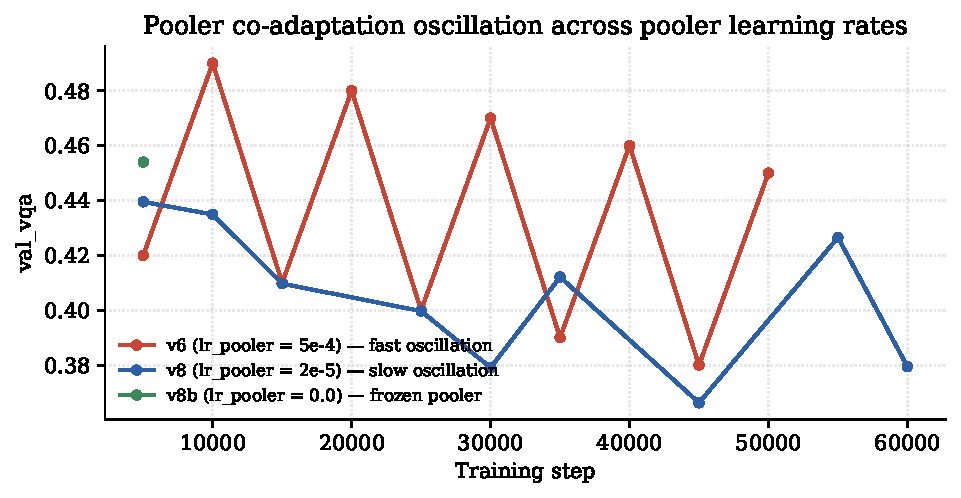
\includegraphics[width=0.95\textwidth]{figures/oscillation.pdf}
\caption{Representative pooler versions from the FM1 sweep.
\emph{Top:} active trainable pooler with $\etasel{=}5{\times}10^{-4}$,
period $\approx 5$K steps. \emph{Middle:} active trainable pooler with
$\etasel{=}2{\times}10^{-5}$, period $\approx 15$K steps.
\emph{Bottom:} frozen pooler, no oscillation but fixed noise tokens the
LLM cannot use.}
\label{fig:oscillation}
\end{figure}

\paragraph{Remedy.}
Replace the trainable bridge with the parameter-free informative token
merge (Section~\ref{sec:merge}). With no learnable connector, one edge of
the gradient circuit is structurally absent and the loop cannot close.
In our LLaVA stack, all active trainable-pooler configurations oscillated;
the frozen bridge did not oscillate but was unusable, and the
parameter-free \textsc{TC-ViTok Final} does not oscillate.

\subsection{FM2: BudgetPredictor Collapse}
\label{sec:fm2}

\paragraph{Prediction.}
\emph{Any adaptive-$k$ head supervised by a monotone-in-$k$ task gradient
and the budget penalty in Eq.~\ref{eq:budget-loss} has a
collapse boundary below which $\keff\!\to\!\kmax$ uniformly, and an
upper region where budget pressure degrades task performance without
necessarily causing collapse. The existence of a non-empty stable
window is the prediction; its location depends on architecture.}

\paragraph{Mechanism.}
The budget head receives two opposing gradient signals: $\Lvqa$ pulls
$\keff$ \emph{up} (more tokens generally ease VQA), $\mathcal{L}_b$ pulls
it \emph{down}. When the former dominates, the predictor converges to the
trivial saturating policy $k_\mathrm{frac}\!\to\!\kmax/N$ uniformly and
the adaptive variant degenerates to fixed-$\kmax$ with a dead-weight
head.

\paragraph{Signature.}
Fine-tuning the adaptive variant from a warm-started base, we observe a
sharp transition (Table~\ref{tab:budget-collapse}). In seed 42,
$\lbb{=}0.03$ collapses to $287.97/288$ within 10K steps and validation
loss regresses; $\lbb\in\{0.08,0.10,0.15\}$ are non-collapsed, and
$\lbb{=}0.20$ enters a stronger budget-pressure regime. Seed-7
replications reproduce the lower collapse at $\lbb{=}0.03$ (final
$\keff{=}288.00$) and the stable region at $\lbb\in\{0.08,0.10,0.15\}$
(final $\keff=281.83,270.37,245.71$). This supports a two-seed
replicated non-empty stable adaptive-budget window, while the high
budget-pressure boundary at $\lbb{=}0.20$ remains single-seed.
Interestingly, seed~7 at $\lbb{=}0.03$ reaches the lowest validation
loss in the table despite saturating at $\keff{=}288$: budget collapse
is a loss of adaptivity, not necessarily a loss degradation.
The low NTP partly reflects its full $k{=}288$ budget; because token
counts and continuation trajectories differ, Val does not rank selector
quality. Adaptive budgeting aims to reduce average token cost below
$\kmax$; collapse reverts to fixed-$\kmax$ and eliminates that saving.

\begin{table}[t]
\caption{BudgetPredictor outcome during fine-tuning of the warm-started
checkpoint. Collapse: $\keff{>}0.99\,\kmax$ for $\geq 2$K consecutive
steps. $\keff$ is the final effective budget; Val is best observed
validation NTP loss, not a direct selector-quality ranking because token
counts and continuation trajectories differ. Seed-7 replications are
completed for $\lbb\in\{0.03,0.08,0.10,0.15\}$; ``n/a'' indicates not
replicated in seed~7. Collapse denotes saturation to the full-budget
policy: the low Val at seed-7 $\lbb{=}0.03$ shows that a collapsed head
can still behave as a strong fixed-full-budget model, but it eliminates
per-sample token reduction below $\kmax$. Stronger budget pressure means
non-collapsed $\keff$ below $\kmax$ with worse Val than the best stable
setting; $\lbb{=}0.20$ remains exploratory and single-seed.}
\label{tab:budget-collapse}
\centering
\small
\renewcommand{\arraystretch}{1.05}
\begin{tabular}{cccl}
\toprule
$\lbb$ & seed-42 $(\keff,\mathrm{Val})$ & seed-7 $(\keff,\mathrm{Val})$ & Outcome \\
\midrule
$0.03$ & $287.97,\;0.3898$ & $288.00,\;0.2466$ & collapsed in both seeds\\
$0.08$ & $280.15,\;0.3368$ & $281.83,\;0.3285$ & stable in both seeds\\
$0.10$ & $271.00,\;0.3177$ & $270.37,\;0.3391$ & stable in both seeds\\
$0.15$ & $247.23,\;0.3176$ & $245.71,\;0.3078$ & stable in both seeds\\
$0.20$ & $227.85,\;0.3291$ & n/a & stronger budget pressure\\
\bottomrule
\end{tabular}
\end{table}

\paragraph{Remedy.}
Operate inside the measured non-collapsed region, with
$\lbb\!\in\![0.08,0.15]$ the two-seed replicated non-collapsed region.
Apply the budget head only on a
converged base. We expect analogous collapse boundaries in other
adaptive-compression systems whenever a budget penalty is the only
counterweight to a monotone-in-$k$ task gradient~\cite{meng2022adavit,rao2021dynamicvit},
but the thresholds in Table~\ref{tab:budget-collapse} are specific to
this stack. The $\lbb{=}0.20$ row represents a higher-pressure regime
that is non-collapsed but has worse Val than the stable region; this
upper zone remains exploratory and single-seed.

\subsection{FM3: Warm-Start Dependence}
\label{sec:warmstart}

\paragraph{Prediction.}
\emph{Joint random-initialisation training of a high-capacity selector
and LLM adapters in the tested 7B-scale stack, supervised by end-task loss
alone, plateaus above any warm-started equivalent unless an additional
supervisory signal (distillation, oracle attention, or a strong prior on
the selector) is introduced. This prediction is the weakest of the three
because the existence of any one effective supervisory augmentation
would falsify it; we invite that test.}

\paragraph{Mechanism.}
A randomly-initialised TPN gives the LLM a near-uniform selection
distribution; LoRA faces a flat task landscape and adapts in directions
that are information-poor for the converged regime. The selector then
receives gradient signal back through a LoRA trained on near-uniform
input. Neither parameter group offers the other useful signal until at
least one reaches a non-trivial regime. The co-adaptation loop is not
oscillating here; it is \emph{stuck}. This places FM3 closer to
curriculum and progressive-training failures~\cite{bengio2009curriculum}
than to FM1's cyclic dynamics.

\paragraph{Signature.}
Across four independent large-scale runs spanning two selector variants,
three LoRA capacities, and four learning-rate regimes, every
from-scratch joint training plateaued well above the warm-started
ceiling (Table~\ref{tab:warmstart}). The only configuration that
approached the ceiling started from a converged base.

\begin{table}[t]
\caption{Warm-start vs.\ from-scratch outcomes on the joint
TPN+LoRA+projector system. Val-VQA is NTP cross-entropy on VQAv2 val
(lower is better).}
\label{tab:warmstart}
\centering
\small
\renewcommand{\arraystretch}{1.05}
\begin{tabular}{lllcc}
\toprule
\textbf{Initialisation} & \textbf{TPN} & \textbf{LoRA $r/\alpha$} & \textbf{Best Val-VQA} & \textbf{Steps} \\
\midrule
warm-start (P1-Final ckpt) & v1 & 64 / 128 & \textbf{0.3177} & 40K \\
from scratch               & v1 & 64 / 128 & 0.4915 (oscillating)            & 48K \\
from scratch               & v3 & 32 / 64  & 0.4380 $\to$ 0.39 (regressing)  & 40K \\
from scratch               & v3 & 32 / 64$^\dagger$ & 0.3334 (still descending) & 50K \\
\bottomrule
\end{tabular}\\[2pt]
{\footnotesize $^\dagger$ Image-only TPN; approached the from-scratch
plateau near Val-VQA $\approx 0.33$ on a single seed by step 50K, not
the warm-started ceiling of 0.3177. Rows 1--2 are the controlled
warm-start comparison; rows 3--4 vary selector variant and LoRA rank
and show the plateau across heterogeneous from-scratch settings.}
\end{table}

\paragraph{Remedy.}
We do not defeat this failure mode. The observed phenomenon is that
from-scratch joint training plateaus above the warm-started ceiling
under end-task supervision alone. Distillation, oracle importance, or
strong selector priors are untested falsification paths rather than
completed mitigations in this paper.
Thus FM3 is reported as an observed training pathology and falsifiable
hypothesis, not as a validated mechanism with a completed mitigation.

\subsection{Reproduction Protocols for Other Architectures}
\label{sec:portability}

Each failure mode carries a reproduction protocol on a different
(encoder, LLM, selector) triple, intended to make the predictions in
Sections~\ref{sec:fm1}--\ref{sec:warmstart} testable by independent
groups without re-deriving the analysis.

\paragraph{Reproduction protocols.}
FM1: instantiate a trainable bridge (learned pooler, cross-attention
summariser, or auxiliary projector) between a frozen visual encoder and
an adapter-trained LLM, sweep selector learning rates over at least one
decade, and test whether oscillation period grows as selector updates
shrink; replacing the bridge with a parameter-free recovery operator
removed the cycle in our stack. FM2: add an adaptive-budget head with penalty
$\lbb\,\mathbb{E}[\keff/N]$, sweep $\lbb$ from $0.03$ to $0.30$, and
test for a collapse boundary below a non-empty stable region. FM3:
train from random initialisation with and without an auxiliary
token-level distillation signal, such as \textsc{LoRA-576}
single-token-ablation importance or CLS-attention scores as soft TPN
targets. FM3 is falsified in this stack if the distillation-augmented
run reaches Val-VQA $\leq 0.33$ within 80K steps, twice the 40K
warm-start horizon; without such a counterexample, the observed gap
remains a warm-start-dependence diagnosis rather than a solved pathology.

% ======================================================================
\section{Experiments}
\label{sec:experiments}

\subsection{Setup}

\paragraph{Hardware and data.}
All experiments run on $2{\times}$ RTX 6000 Ada (49\,GB each) with
PyTorch DistributedDataParallel (DDP), BF16 mixed precision, and
effective batch size 128. We train on
VQAv2~\cite{goyal2017vqav2} and GQA~\cite{hudson2019gqa} and evaluate on
VQAv2 val2014, GQA val\_balanced, POPE~\cite{li2023pope}, MMBench English
dev, and TextVQA val.

\paragraph{The missing control.}
Comparing a LoRA fine-tuned compressive system against an off-the-shelf
uncompressed baseline conflates compression with LoRA effects. We
introduce \textsc{LoRA-576}: the same Phase-1-Final LoRA adapter and
multimodal projector evaluated with all 576 tokens forwarded to the
LLM, byte-identical to \textsc{TC-ViTok Final} in rank, alpha,
dropout, targets, SFT data, optimiser, and checkpoint step. The
architectural comparison is \textsc{TC-ViTok Final} versus
\textsc{LoRA-576}, both at $\sim\!60$~GPU-h compute; published
query-agnostic methods are not compute-matched. This control isolates
compression cost from fine-tuning effects, a confound often left open
when compression papers compare only to released full-token checkpoints.

\subsection{Main Results}
\label{sec:main-results}

\textsc{TC-ViTok Final} costs $-4.1/-3.4/-7.4$~pp on VQAv2/GQA/POPE
against \textsc{LoRA-576} (Table~\ref{tab:main}). The same pattern
persists on an independently retrained seed
(Table~\ref{tab:seed-replication}): the gap is not a seed-42 artefact.
Against published query-agnostic methods, \textsc{TC-ViTok}
underperforms by $\sim$5 points; those methods use the full publicly
released LLaVA-1.5 SFT mix that \textsc{LoRA-576} also lacks, so the
compute-matched architectural cost is the gap to \textsc{LoRA-576}.

\paragraph{Trivial-selector baselines.}
We evaluate three trivial selectors at the same $k{=}144$, same LoRA
adapter, and same hard-drop path: uniform random selection, uniform
grid (every 4th patch), and CLS-attention top-$k$ on CLIP's last
layer (Table~\ref{tab:main}). \emph{The learned TPN does not surpass
the strongest trivial baseline on any of VQAv2, GQA, POPE, MMBench,
or TextVQA.} On VQAv2, GQA, and TextVQA the TPN loses to all three
trivial selectors. On POPE it marginally exceeds CLS-attention top-$k$
($79.09$ vs.\ $78.94$) but falls well short of random ($83.92$) and
grid ($82.78$). On MMBench it beats random and uniform grid but trails
CLS-attention top-$k$ by $0.05$~pp ($62.0$ vs.\ $62.05$), a difference
within binomial noise (SE $\sim$2.5~pp), so we treat the two as
statistically indistinguishable. The
TextVQA gap is the most striking instance: CLS-attention top-$k$ on
the same $24{\times}24$ patch grid exceeds the TPN by $10.8$\,pp,
indicating that the joint-training objective did not refine the
selector toward text-localisation regions even though that prior is
present in CLIP's last-layer attention. The overall pattern is
consistent with, but does not independently establish, FM3
(warm-start dependence): the ceiling we approach is bounded by what
trivial selection already extracts from this LoRA adapter, and joint
end-task supervision through the LLM does not push the learned
selector beyond that ceiling. Section~\ref{sec:discussion} gives a
compact probe analysis supporting this diagnostic interpretation.
For VQAv2 and GQA, the gaps to the strongest trivial selector
($2.64$ and $3.28$~pp) are far larger than the corresponding binomial
standard errors ($0.16$ and $0.22$~pp).

\paragraph{Scaling with token budget.}
The negative finding extends across budgets. On the Phase~1 Adaptive
checkpoint, evaluating the same four selectors at
$k\!\in\!\{36,72,144,216,288\}$ shows that the learned TPN does not
beat the strongest trivial baseline at any measured $k$ on VQAv2, GQA,
or POPE (Fig.~\ref{fig:k-scaling}). The gap narrows as $k$ increases
but does not reverse, supporting the interpretation that joint
end-task supervision through the LLM fails to outperform trivial
selection in this regime rather than only at the headline
$k{=}144$; the failure is not specific to one operating point.

\begin{figure}[t]
\centering
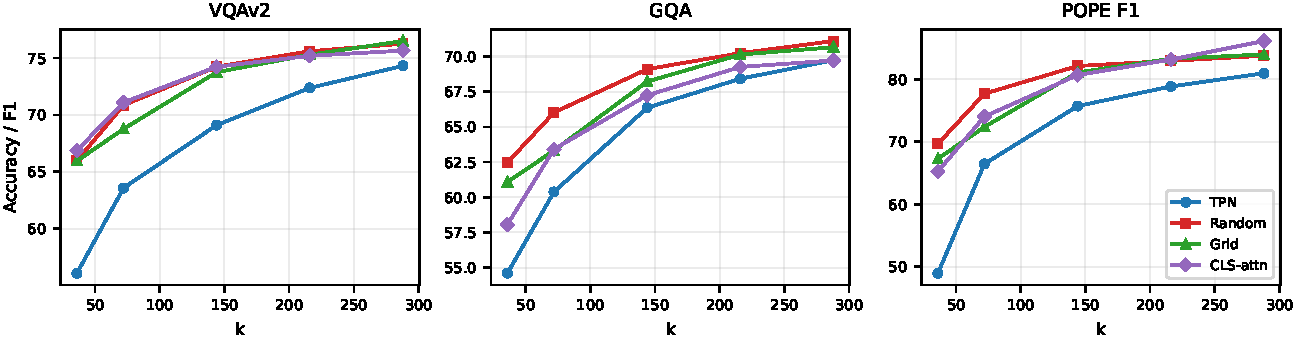
\includegraphics[width=0.84\textwidth]{figures/k_scaling.pdf}
\caption{Token-budget sweep on the Phase~1 Adaptive checkpoint. The
learned TPN remains below the strongest trivial selector at every
measured $k$ on VQAv2, GQA, and POPE; ``strongest'' is the per-$k$
maximum of random, grid, and CLS-attention top-$k$.}
\label{fig:k-scaling}
\end{figure}

\begin{table}[t]
\caption{Main results on LLaVA-1.5-7B. Headline comparison is
\textsc{TC-ViTok Final} vs.\ \textsc{LoRA-576}. All \textsc{TC-ViTok}
rows are single-seed evaluations; binomial standard errors at the
listed sample sizes are $\sigma{\approx}0.16$~pp for VQAv2 testdev,
$\sim$0.22~pp for GQA, $\sim$0.50~pp for the 5K POPE subset,
$\sim$2.5~pp for MMBench dev, and $\sim$0.7~pp for TextVQA val.
``n/a'' means not evaluated.}
\label{tab:main}
\centering
\small
\renewcommand{\arraystretch}{1.05}
\setlength{\tabcolsep}{2.5pt}
\begin{tabular}{lcccccc}
\toprule
\textbf{Method} & \textbf{Tok} & \textbf{VQAv2} & \textbf{GQA} & \textbf{POPE F1} & \textbf{MMB} & \textbf{TextVQA} \\
\midrule
\multicolumn{7}{l}{\emph{Published (LLaVA-1.5 SFT, no extra LoRA):}} \\
LLaVA-1.5-7B (full)~\cite{liu2024llava} & 576 & 78.5 & 61.0 & 84.4 & 64.3 & 58.2 \\
\midrule
\multicolumn{7}{l}{\emph{Same-LoRA reference and ours (this work, $\le$80K steps):}} \\
\textsc{LoRA-576} (control)         & 576       & 76.38 & 70.55 & 86.46 & 61.7 & 38.4 \\
\textsc{TC-ViTok} v3 (hard drop)    & 144       & 72.47 & 59.87 & 78.50 & n/a & n/a \\
\textsc{TC-ViTok} Adaptive          & 36--288   & 69.43 & 65.04 & 75.63 & n/a & n/a \\
\textbf{\textsc{TC-ViTok} Final}    & \textbf{144} & \textbf{72.27} & \textbf{67.12} & \textbf{79.09} & \textbf{62.0} & \textbf{25.8} \\
\quad merge disabled at eval        & 144       & 72.27 & 67.12 & 79.09 & n/a & n/a \\
\quad zero CLIP query at eval       & 144       & 72.67 & 67.45 & 79.37 & n/a & n/a \\
\midrule
\multicolumn{7}{l}{\emph{Trivial-selector baselines (same LoRA, $k{=}144$, hard drop):}} \\
Random drop                         & 144       & 74.05 & 70.40 & 83.92 & 61.24 & 29.63 \\
Uniform grid                        & 144       & 74.65 & 69.26 & 82.78 & 61.93 & 29.61 \\
CLS-attention top-$k$               & 144       & 74.91 & 68.16 & 78.94 & 62.05 & 36.57 \\
\midrule
\multicolumn{7}{l}{\emph{Published query-agnostic methods (different SFT mix and compute):}} \\
FastV~\cite{chen2024fastv}              & 144       & 77.1 & n/a & n/a & n/a & n/a \\
LLaVA-PruMerge~\cite{shang2024llava}    & 144       & 76.8 & n/a & n/a & n/a & n/a \\
SparseVLM~\cite{zhang2025sparsevlm}     & ${\sim}152$ & 78.2 & n/a & n/a & n/a & n/a \\
\bottomrule
\end{tabular}
\end{table}

\begin{table}[t]
\caption{Two-seed replication of the matched compression gap. Rows are
5K-sample evaluations from the validation sets at the Phase-1 Final
checkpoint (80K steps, identical configuration).}
\label{tab:seed-replication}
\centering
\small
\renewcommand{\arraystretch}{1.05}
\begin{tabular}{llccc}
\toprule
\textbf{Seed} & \textbf{Model} & \textbf{VQAv2} & \textbf{GQA} & \textbf{POPE F1} \\
\midrule
42 & \textsc{TC-ViTok} Final & 72.27 & 67.12 & 79.09 \\
42 & \textsc{LoRA-576}       & 76.38 & 70.55 & 86.46 \\
 7 & \textsc{TC-ViTok} Final & 72.34 & 67.58 & 78.87 \\
 7 & \textsc{LoRA-576}       & 76.65 & 71.36 & 86.78 \\
\bottomrule
\end{tabular}
\end{table}

\subsection{Properties of the Converged Selector}
\label{sec:selector-properties}

\paragraph{Query-agnostic convergence at inference.}
Zeroing the CLIP query embedding at inference yields
$+0.40/+0.33/+0.28$~pp on VQAv2/GQA/POPE on the Final checkpoint
(Table~\ref{tab:main}); \textsc{Adaptive v2} repeats the sign on two
of three benchmarks, with a marginal GQA reversal. The CLIP query
channel is not useless during optimisation: image-only and
query-conditioned from-scratch runs follow different trajectories in
Table~\ref{tab:warmstart}. At convergence the learned spatial bias
suffices and the query becomes redundant. That removing the query
improves accuracy indicates that joint
optimisation encoded image-distribution priors rather than
question-specific routing. We frame this as a trajectory-internal
property of training on global-image-distribution data (VQAv2, GQA);
independent seeds were not tested.

\paragraph{Token merge: architectural, not benchmark-improving.}
The merge-disabled ablation (Table~\ref{tab:main}) is byte-identical
to the merged result, and a four-point inference-time $\beta$ sweep on
a 5K subset stays within subset noise. The merge's contribution is
\emph{architectural}: it eliminates the trainable bridge that produces
FM1 (Section~\ref{sec:fm1}), not downstream accuracy.

% ======================================================================
\section{Discussion}
\label{sec:discussion}

\paragraph{Why \textsc{TC-ViTok} loses to its matched baseline.}
Three observations explain the $-4.1/-3.4/-7.4$-point gap. First, the
selector's gradient signal arrives via a 32-layer LLM and a frozen
projector; in contrast to systems that distil from a strong
teacher~\cite{rao2021dynamicvit}, our selector is supervised only by
the end-task cross-entropy, a distal signal. Second, the merge $\beta$
sweep (Section~\ref{sec:selector-properties}) shows LoRA absorbs the
merge's information flow at every tested $\beta$; the LLM adapts to
the post-merge representation, shadowing the merge's accuracy
contribution.
Third, pre-LLM compression cannot exploit the early-layer attention
mixing that mid-LLM methods like FastV~\cite{chen2024fastv} rely on:
information lost before layer 0 is lost for all 32 layers, and the
selector must anticipate the LLM's needs without ever seeing an LLM
activation. The TextVQA result is not a grid coarseness ceiling:
CLS-attention top-$k$ reaches $36.57$ at $k{=}144$
(Table~\ref{tab:main}), indicating that end-task training did not
move the selector toward CLIP's text-localisation prior.

\paragraph{Supporting probe evidence for the selector ceiling.}
If learned selection is to improve over trivial baselines by
identifying tokens the LLM will causally use, the representations
available to the selector should contain recoverable per-token
importance. We test this in a matched frozen-teacher probe, using
\textsc{LoRA-576} single-token-ablation loss changes on GQA as a
$1000{\times}576$ target. Under linear/MLP probes, CLIP ViT-L/14
($R^2{=}{-}0.04/{-}0.33$) and DINOv2-large~\cite{oquab2023dinov2}
(${-}0.08/{-}0.30$) do not recover the target; $R^2{<}0$ means
worse-than-mean prediction. The same pipeline recovers row/column
coordinates ($R^2{=}0.39$--$0.52$). A token-permuted CLIP null gives
the same negative pattern ($-0.05/-0.31$). At the FastV-relevant L2
depth, visual tokens receive ${\sim}89\%$ of attention mass, yet
text-to-visual attention is at the mean-prediction baseline
($R^2\!\approx\!-0.02$, $N{=}100$ pilot smoke test). We report this as a
supporting diagnostic result under the tested probes, representations,
and sample sizes. Coordinate prediction is a simpler 2D spatial target
than 576-way token importance; the positive control validates the
pipeline, not the hardness of the target. The result does not rule out
weaker signals, richer probes, larger datasets, or alternative
causal-importance targets.

\paragraph{Limitations.}
(1)~Primary failure-mode evidence comes from one LLaVA stack; the
Qwen2-VL-7B portability attempt did not reach non-trivial task accuracy.
(2)~The headline rows are single-seed, although one independently
retrained seed checks that the compression gap is not unique to seed 42;
we do not claim statistical significance across random initialisations.
FM2's lower collapse and stable region are replicated through $\lbb{=}0.15$, while the
$\lbb{=}0.20$ budget-pressure row remains single-seed. (3)~The gap to
\textsc{LoRA-576} is not closed, and learned selection never surpasses
the strongest trivial selector across our $k$ sweep. (4)~The
$\Tosc(\etasel)$ relation is a trajectory-level diagnostic, not a
scaling law. (5)~The probe analysis is scoped to one VLM, one benchmark,
two encoder families, linear/MLP probes, $N{=}1000$ encoder probes, and
an $N{=}100$ attention smoke test. (6)~FM3's distillation-based
falsification criterion is not tested here; the failure mode is
characterised but not solved.

% ======================================================================
\section{Conclusion}

\textsc{TC-ViTok} was built to test a natural idea: train a
query-conditioned selector to keep only the visual tokens the LLM
needs for the current question. In one controlled LLaVA-1.5-7B stack,
the idea fails informatively: the learned selector loses both to
the matched no-compression LoRA-576 reference and to the strongest
question-blind trivial selector on every benchmark we measure. We used
that failure as a diagnostic substrate and observed three optimisation
pathologies in the same stack: co-adaptation oscillation,
BudgetPredictor collapse, and warm-start dependence. The
$\tau$-independent gradient route, parameter-free informative token
merge, and three-stage curriculum are engineering responses that make
the diagnostic system trainable; they do not close the accuracy gap.
Supporting probes do not recover single-token ablation importance
under the tested settings. Evidence is from one stack; the failed
Qwen-VL portability attempt is not validation, so the main output is a
controlled negative result plus falsifiable hypotheses for independent
stacks. In stacks similar to the one studied here, practitioners should
first compare against matched CLS-attention or uniform-grid compression
baselines before investing in joint pre-LLM selector training under
end-task supervision alone.

% ----------------------------------------------------------------------
\bibliographystyle{splncs04}
\bibliography{main}

\end{document}
